\chapter{Requirements and Analysis}

\section{Detailed Problem Statement}
%% TODO
This project aims to implement a library of reusable verified distributed components,
based on the classical family of fault-tolerant asynchronous Paxos-like consensus protocol.
The project will use Disel, a framework for compositional verification of distributed
protocols built on top of the Coq proof assistant, to verify correctness of the
implemented components.

\section{Requirements}
\begin{enumerate}
  \item Adapt Paxos for encoding in Disel and devise the state-transition system for this protocol.
  \item Develop an inductive invariant for the adapted protocol that
    ensures the protocol functions correctly by imposing requirements on the global state of the system
  \item Implement a simulation of the adapted protocol with the developed state transition system.
  \item Mechanise the proof of the adapted protocol in Disel/Coq.
    Thereby, providing a library of reusable verified distributed components.
  \item Mechanise a client application of the protocol verified out of the abstract interface.
\end{enumerate}

\vspace{-5mm}
\section{Analysis: Approach to Mechanising Proofs in Disel}
Having decided on the requirements we came up with a workflow to
mechanise the proof in Disel.

\begin{figure}
\centering
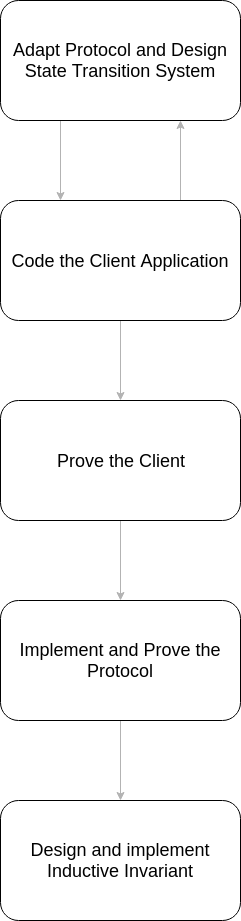
\includegraphics[width=0.2\textwidth]{figures/disel_workflow.png}
\caption{Disel Workflow
\label{fig:myInlineFigure}}
\end{figure}

% (1) Write code before proofs and run/test it;
%         (2) Prove that the code follows the protocol;
%         -----
%         (3) Write the protocol and prove invariants;
%
%
% You might want to have a diagram for this…
%
% Take a look at this paper (without going into details):
%
% https://www2.eecs.berkeley.edu/Pubs/TechRpts/2017/EECS-2017-163.pdf
%
% You might want to make a point that even without verifying inductive invariants, we already can get relatively strong correctness properties just by verifying (1)-(2).
%
% (1)-(2) is also sort of delivered by this work: https://eb.host.cs.st-andrews.ac.uk/writings/tdd-conc.pdf
%
% 1. I suggest you first
%   give a textual description with a lot of intuition about what kind of client
%   we are interested in and what properties it can observe that are guaranteed by the consensus.
% 2. Then you specify this property formally and sketch its proof.
%
% The client application does only need to have a couple of RPC-like procedures.
% It doesn't have to know about the entire protocol.
%
% Adapt Protocol and Design State transition system (iterate)
% | |
% Design and implement the Client Application (iterate)
% |
% Prove Client
% |
% Implement and prove Protocol
% |
% Prove the Inductive Invariant

\subsection{Adapt protocol and design state transition system}
By adapting the protocol we try to focus on the 'core' parts of the protocol
and to do away with the 'conveniece' parts. For Paxos, this was focusing on the
part of the protocol that deals with achieving consensus and not looking at the
part where the learner is informed of the decision.

We also need to design state transition systems for the nodes that participate
in the protocol. This makes it easier for us to encode the protocol in Disel as
we already know which send and receive transitions we will need from each state
and thus can easily code the transition wrappers.

In chapter 4, we look go into the details of how we tackled this stage on our way
to mechanising the proof of Paxos.

\subsection{Code the client application}
Secondly, we need to think of a client application that uses the implemented protocol.
We need to design and implement a client that will demonstrate the properties of the
protocol that we want to prove. In case of Paxos, we designed a client
where nodes try to acheive consensus on one of the proposals that the proposer
is initialised with. This enabled us to see in action the stages of the protocol
that lead to consensus being achieved.

While using Disel, we often had to cycle between stage 1 and stage 2.
This is because while implementing the client, you realise things like, you are
missing one state for a node that is required in order for the protocol to progress.
While writing the client for Paxos, we realised that we were missing the \texttt{PAbort}
state for the proposer, which was necessary to signify when a proposer stops
participating in the protocol.

The process of cycling between stages 1 and 2 allow us to solidify our adapted
protocol. Doing this at an early stage (before starting the proofs)
also has the advantage of us not having to rewrite a lot of code that will also
break all the proofs relating to the change.

Additionally, implementing the client also helps us identify unnecessary stages
and transitions in the adapted protocol which were not needed to implement the
client. Reducing the number of states and transitions vastly reduces the amount
of things you will need to prove in the later stages.

\subsection{Prove the client}
The next stage involves proving that the code for the client actually follows
the adapted protocol. Thus, finishing the proofs in this stage gives us
confidence that our adapted protocol can actually be used to fullfill the role
which our client performs. In case of Paxos, this helped us realise that our
adapted protocol can be used to achieve consensus among the acceptors.

From this stage onwards, as we move to stages 4 and 5 we end up strengthening
the proof of our protocol. Finishing stage 4 completes the proof of the protocol
while reaching stage 5 actually adds an inductive invariant that stregthens the
proof of the protocol even further.

\subsection{Encode and prove the adapted protocol}
Having proved that client follows the protocol, the next stage is
to actually finish the implementation of the protocol and to prove it. Finishing
stage 3, helped us be sure that the state transitions we have are enough for
realising the `core' part of the protocol and that action of the client is proved.
Now we need to prove the protocol itself.

Finishing this stage meant that we have finished the proof of the protocol,
although we can only be sure that ...

In the proof of Paxos, we were only able to finish still stage 4. We designed
the inductive invariant but ran out of time to prove it.

\subsection{Prove the inductive invariant}

% The analysis part of the chapter is what you did to map the requirements
% information into the first pass design. You can think of analysis as the
% first stage of design, and the purpose is to show how the requirements
% were used to inform the design.

%% TODO: Talk about mapping to Disel Workflow and outline the process followed.

% \subsection{Requirement 1: Adapted Protocol and State Transition System}
% In order to mechanise the proof of Paxos in Disel, we had to first adapt the
% protocol in order to simplify the proof. There are many variants of Paxos and
% we had to study the we decided to focus on single decree paxos, the variant that
% was first proposed by Leslie Lamport %% TODO: Reference
%
% We studied the protocol in detail and also decided to focus on proving the
% part of the protocol that deals with achieving consensus, which is also the
% main function of the protocol. For this reason we did not include the learner
% in our client application or adapted protocol, nor did we focus on the part
% where the chosen value is learnt by all the nodes. We instead let our inductive
% invariant handle the case to detect when consensus had been achieved as the
% inductive invariant can impose requriements on the global system state.
%
% Additionally, we also had to create a state transition system for the nodes in
% the protocol as Disel relies on this to impose pre and post conditions on the
% states of a node. In Paxos
% each node can have different roles but we had to split up each role into different
% states depending on the current data held by the node and the current function
% ofthe node in the protocol. We decided on the states each node could be in and
% how and when it transitions between them. This helped us come up with precondition
% and postcondition for the state of each node when it transitions on receiving or
% sending a message. We tried to minimise the number of transitions and the data
% held in each node’s state in order to simplify the proof in Disel.
%
% We look at these in more detail in the next chapter when we talk about modelling
% the protocol.
%
% \subsection{Requirement 2: Inductive Invariant}
% We also had to come up with an inductive invariant for the protocol such that if
% the inductive invariant holds in some state then in holds in every state reachable
% from that state. The inductive invariant was critical as it helped ensure that
% the protocol functions correctly by imposing requirements on the global state of
% the system. For proving the correctness of paxos we found that our invariant had
% to capture when consensus is achieved on a value and also that once consensus is
% achieved on a particular value, further rounds of the protocol don’t change this
% value. We then also came up with a proof for how this inductive invariant holds
% in our adapted protocol.
%
% \subsection{Requirement 3: Simulation}
% I also needed to implement a simulation of our adapted protocol. The simulator
% must be based on a state-transition system like Disel and should be able
% to simulate different nodes in the distributed system. The main reason for
% implementing this simulation is to be sure that our adapted protocol, designed
% in Requirement 1, will actually be provable in Disel. The simulation will enable
% us to detect errors and fix them much faster than having to fixing them in the
% middle of the Disel proof which is a much more time consuming to implement.
% The simulator will be implemented with the same state transitions we decided
% upon in Requirement 1, thus, the corrent working of the simulator will give us
% confidence that our state transition system for Paxos will work correctly in Disel.
%
% I decided to use Python to implement the simulation as that was the language I
% was strongest in. I studied how the simulation for Multi Paxos was implmented
% in the Paxos made moderately complex paper, %% TODO: Reference
% which helped me learn how to create separate process for each node and also how
% to communicate by exchanging messages between the processes.
%
% \subsection{Requirement 4: Proof}
% Having designed the state transition diagram and the inductive invariant,
% the task of mechanising the proof in Disel becomes much easier.
% For implementing the proofs, I needed to learn more about Coq and SSReflect.
% I had to study examples of protocols proved in Disel, like the proof of the
% Two Phase Commit protocol.
%
% \subsection{Requirement 5: Client Application} %% TODO
% After studying the Disel paper and looking at similar examples, I implemented the
% core of the adapted protocol in Disel. I also implemented a client application in
% Disel. The pre and post conditions from the state transition system helped me to
% implement the client application in such a way to adhere with the main protocol.
% Using the extraction feature in Disel and the shims runtime, I successfully
% extracted a working program of the client application in OCaml.
